
%\newpage
\section{Funkce autotestu}
\label{sec:selftest}
Počínaje verzí 0.9k jsem vytvořil funkci automatického testu.
Použití je snadné.
Propojte všechny svorky kouskem neizolovaného drátu a stiskněte tlačítko start.
Program zjistí zkratované piny a zobrazí zprávu: Autotest..?
Test začne, pokud to do dvou vteřin potvrdíte stisknutím tlačítka start.
Toto potvrzení je nutné aby tester nezačínal samočinně autotest při měření proraženého rozbitého tranzistoru.
Po dokončení samočinného testu, pokračuje přístroj v normálním měření.
Pokud není připojena žádná součástka, končí tester se zprávou ,,žádná neznámá vadná součástka''.
Funkci autotestu můžete zvolit pouze pro ATmega168 nebo ATmega328.
Před provedením dalších testovacích kroků je nejprve nastaven nulový odpor pro všechny tři kombinace testovacích pinů
(T1:T3, T2:T3 a T1:T2). Tyto nulové odpory se používají pro budoucí měření ESR a odporů pod \(10\Omega\).
Akceptovány jsou pouze nulové hodnoty odporů pod \(0.90\Omega\), protože tyto korekční hodnoty jsou při měření odporů přes \(10\Omega\) přehlédnuty.
Při změně používaných kabelů musí být proto zajištěno dodržení nízké hodnoty odporu.
Jestliže později klesnou hodnoty odporů naměřené pod příslušný nulový odpor o více
než \(0,2\Omega\) je tester resetován na ,,Nezkalibrováno!''.
To je indikováno aktivovaným kurzorem při testu.
Jednotlivé kroky funkce automatického testu týkající se testu 1 až test 7 jsou zobrazeny v prvním řádku LC displeje s písmenem T následovaným číslem kroku.
Kroky 1 až 7 se opakují čtyřikrát, než se program dostane k dalšímu kroku.
Pokud však po dokončení kroku stisknete tlačítko Start, nebude se tento test znovu opakovat.
Pokud držíte tlačítko stisknuté během celého automatického testu, bude každý krok proveden pouze jednou.
Bez možnosti AUTO\_CAL se v každém kroku zobrazí pouze výsledky měření, není provedena žádná analýza chyb.
Výsledky musíte vyhodnotit sami.
V tomto okamžiku bych chtěl dát důležitou radu.
Nikdy neprovádějte měření a kalibraci při připojení k ISP konektoru! Rozhraní ISP zasahuje do měření.

\vspace{1cm}
Zde je seznam aktuálně nainstalovaných testů:
\vspace{1cm}

\begin{enumerate} \setlength{\itemsep}{0em}

\item \textbf {Měření \(1,3V\) (nebo \(1,1V\)) velikost referenčního pásma (band gap Reference).}
\\V řádku~1 je text ,,Ref='' měřené napětí zobrazené v mV.\\
U měniče ATmega8 by měřené napětí mělo být blízké \(1,3V\), u ostatních procesorů je referenční napětí normálně kolem \(1,1V\).

Druhý řádek ukazuje výsledný faktor měření kapacity s \(470k\Omega\) odporem.

\item \textbf {Porovnání \(680\Omega\) odporů.} 
V prvním řádku se zobrazí kryptický text  ,,+RL- 12 13 23''.
To znamená:
RL je zkratka pro (Rezistor Low = nízký odpor), což znamená \(680\Omega\) odpor. ,,12'' znamená: 
Odpor na pinu~1 je připojen k VCC (+) a odpor na pinu~2 je připojen k GND (-).
Výsledek tohoto měření stojí v 2~řádku na prvním místě jako rozdíl teoretické hodnoty.
V řádku~1 nyní následuje ,,13'', což znamená, že odpor pin-1 je opět připojen k VCC,
ale nyní je na GND připojen \(680\Omega\) odpor pinu~3.
Výsledek je v 2~řádku na prostředním místě jako rozdíl k teoretické hodnotě.
Poslední měření této zkoušky ,,23'' znamená, že odpor pinu~2 je nyní připojen k VCC a
odpor pinu~3 je připojen k GND.
Výsledek je poslední ve druhé řádce LCD jako rozdíl teoretické hodnoty.
Chtěl bych připomenout, že ADC rozlišení je asi \(4,88mV\)!
Situace měření je také zobrazena na obrázku~\ref{fig:test2}.
Teoretická hodnota s ohledem na odolnost vnitřního portu je následující:
\(\frac{5001 \cdot  (19+680)}{ (19+680+680+22)} = 2493\).
\begin{figure}[H]
  \begin{overpic}[width=1.\textwidth]{../FIG/Test2.pdf}
  \color{black}
  \put(18,22){\makebox(0,0)[cb]{první měření}}  
  \put(49,22){\makebox(0,0)[cb]{druhé měření}}  
  \put(85,22){\makebox(0,0)[cb]{třetí měření}}  
  \end{overpic} 
  \caption{Porovnání \(680\Omega\)-odporů}
  \label{fig:test2}
\end{figure}
\item \textbf {Porovnání \(470k\Omega\) odporů.}\\
Nyní se na displeji zobrazí řádek 1 ,,+RH- 12 13 23''.
Stejný postup jako v kroku~2 se opakuje s \(470k\Omega\) odpory (Symbol RH).
Výsledky jsou prezentovány jako rozdíl pro \(\frac{VCC \cdot (19 + 470000]}{ (19 + 470000 + 470000 + 22)} \)
pro všechny kombinace.

\item  V tomto kroku není nic měřeno, pouze \textbf {příkaz ,,Isoluj sondy!''},
což znamená, že je čas odpojit svorky (odpojení holého drátu).\\
Tento krok je dokončen pouze v případě, když jste rozpojili testovací piny (porty).

\item Tento krok testuje \textbf {schopnost na GND (-) připojení \(470k\Omega\) odporů (H) zkušebních pinů na GND.}\\
Řádek 1 zobrazuje text ,,RH-''.\\Řádek 2 by měl vykazovat nulovou hodnotu \(mV\) pro všechny tři piny.

\item Tento krok zkouší \textbf {schopnost s VCC (+) spojené \(470k\Omega\) odpory (H) zvednout testovací piny na VCC.}\\
Řádek 1 zobrazuje text ,,RH+''.
Nejlepší možná hodnota pro tři měření by měla být v 2~řádku  \(0mV\), protože rozdíl je reprezentován jako VCC.
\\Velké odchylky od ideální hodnoty pro kroky 5 a 6 jsou chyby, jako je problém s izolací, svodový proud nebo poškozený testovací pin (port).

\item \textbf {Tento krok testuje napětí napěťového děliče \(470k\Omega / 680\Omega\).}\\
Řádek 1 zobrazuje text ,,RH/RL''.
Řádek 2 ukazuje odchylku od očekávaného napětí dělitele \(470k\Omega\) / \(680\Omega\) \(5V\) u všech tří zkušebních pinů. Odchylky více než několika mV indikují chybu při montáži odporů.

\item \textbf {Měření vnitřních odporů s GND spojených výstupů.}\\
Tento a následující kroky se provádějí pouze při volbě možnosti AUTO\_CAL.
Vnitřní Port-C odpory od na GND (-) připojených výstupů budou měřeny proudem
procházejícím \(680\Omega\) odpory které wedou k VCC (+), viz obrázek~\ref{fig:test7}.
Měřeny jsou pouze ty tři piny ADC portu, odporové porty PB0, PB2 a PB4 nelze měřit bez změny hardwaru.
Předpokládá se, že odolnost různých portů je téměř identická.
Hodnota odporů je uvedena v dalším kroku.
\begin{figure}[H]
\centering
  \begin{overpic}[width=.9\textwidth]{../FIG/Test7.pdf}
  \color{black}
  \put(16,34){\makebox(0,0)[cb]{první měření}}  
  \put(49,35){\makebox(0,0)[cb]{druhé měření}}  
  \put(85,35){\makebox(0,0)[cb]{třetí měření}}  
  \end{overpic}
  \caption{Měření vnitřního odporu výstupů portu C připojených k GND}
  \label{fig:test7}
\end{figure}

\item \textbf {Měření vnitřních odporů s VCC spojenými výstupy portu MCU.}\\
Požadovaný proud je dodáván přes GND spojených \(680\Omega\)-odporů.
Je to stejné měření jako měření v testu 8 na druhé straně, jak je ukázáno na obrázku \ref{fig:test8}.
\\Interní odpor se vypočítá následovně:
\\Pro výpočet proudu: \((5001 - (výsledekt~testu~8) - (výsledekt~testu~9)) / 680\).
\\Hodnoty odporu se získají, když je naměřené napětí dělením tohoto proudu.
\\Výsledek tohoto testu se pak zobrazí v řádku~1 s textem ,,RI\_Hi='' in \(\Omega\),
\\vnitřní odpor na stránce GND se zobrazí v řádku~2 s textem ,,RI\_Lo=''.
\\Od softwarové verze 1.06k jsou tyto hodnoty při každém měření nově určeny a zde se pouze zobrazují.

\begin{figure}[H]
\centering
  \begin{overpic}[width=.9\textwidth]{../FIG/Test8.pdf}
  \color{black}
  \put(16,35){\makebox(0,0)[cb]{první měření}}  
  \put(49,35){\makebox(0,0)[cb]{druhé měření}}  
  \put(85,35){\makebox(0,0)[cb]{třetí měření}}  
  \end{overpic}
  \caption{Měření vnitřních odporů s VCC a spojenými výstupy portu C}
  \label{fig:test8}
\end{figure}

\item \textbf {Měření nulového ofsetu při měření kondenzátorů.}
\\Pro pinové kombinace 1:3, 2:3 und 1:2 je nulová hodnota měření kondenzátorů v \(pF\) v řádku~1
za textem  ,,C0 ''.
V softwaru se pro normální výstup měření bere v úvahu výchozí hodnota přibližně \(39pF\).
Pro výstupek této zkoušky se nezohledňuje žádná korekce, není odečtený žádný nulový ofset.
Rovněž jsou určeny nulové odchylky pro reverzní pinovou kombinaci.
Nalezené nulové odchylky jsou uloženy v EEPROM, pokud jsou všechny nulové ofsety menší než \(190pF\).
Na řádku 2 se zobrazí ,,OK''.
Nalezené nulové odchylky jsou vzaty v úvahu pro další měření kapacity v závislosti na pinu.
Sleduje se, zda měřená kapacita klesne pod zaznamenanou nulovou kapacitu o více než \(20pF\).
Pokud by se tak stalo, je tester resetován na ,,nezkalibrovaný''.
To je indikováno aktivací kurzoru LCD (kurzor) při příštím testu.
Vezměte prosím na vědomí, že pokud se změní nastavení měření, má smysl nový autotest.
Nulový ofset může být, při použití kabelů, přibližně o \(3pF\) vyšší ve srovnání se svorkami.
Pokud byl testovací přístroj konfigurován s funkcí SamplingADC přidá se, pro metodu měření ADC vzorkování, měření nulové kapacity v dvojnásobném počtu konfigurací.
Je to proto, že je nulová kapacita určena ve všech pinových kombinacích jak pro nabíjení tak i pro vybíjení.

\item {\textbf {Čekání na připojení kondenzátoru na pin~1 a pin~3.}}
\\Na 1 řádku displeje se zobrazí zpráva ,,\mbox{\begin{large}1 \electricC 3 ~\textgreater 100nF\end{large}}''.
K připravení měření napěťového ofsetu analogového komparátoru musí být dostatečně velký
kondenzátor připojený mezi piny 1 a 3.
Měl by to být vysoce kvalitní kondenzátor s kapacitou mezi \(100nF\) a \(20\mu F\). 
Za žádných okolností byste neměli používat elektrolytické kondenzátory.


\item \textbf {Měření ofsetu komparátoru pro nastavení měření kondenzátorů.}
\\Pro určení offsetu analogového komparátoru musí být kondenzátor připojen na pin~1 a pin~3.
Kondenzátor je potřebný pro vyrovnávání nabíjecího napětí při měření kondenzátorů k určení rozdílu mezi
nabíjecím napětím a vnitřním referenčním napětím.
Pokud je měření úspěšné, zobrazí se korekční hodnota krátce  na 1 řádku s textem ,,REF\_C='' a bude zapsaná do EEPROM paměti.
Pokud jste vybrali volbu AUTOSCALE\_ADC bude zesílení funkce čtení ADC porovnáno s nastaveným vnitřním referenčním napětím.
To se provádí porovnáním napětí kondenzátoru pod \(1V\),  jednou s VCC referencí a jednou s interní referencí.
Nalezený rozdíl je zobrazen ve 2 řádku s textem ,,REF\_R='' a bude také zaznamenán v paměti EEPROM.
Hodnota REF\_R\_KORR je pak pouze dodatečným ofsetem pro tento automaticky zjištěný rozdíl.

\item {\textbf {Čekání na kondenzátor k měření malých indukčností}}
\\Pokud je tester nakonfigurován s funkcí SamplingADC je pro měření malých indukčností
kondenzátor se známou velikostí potřebný pro výpočet indukčnosti z kmitočtu rezonance.
Užitečné hodnoty kapacity jsou asi \(10nF\) až \(27nF\).
Vhodný kondenzátor by měl být připojen na pin~1 a pin~3, pokud se na 1 řádku objeví zpráva ,,\mbox{\begin{large}1 \electricC 3~10-30nF(L)\end{large}}''.
{\textbf Přesně tento kondenzátor} by pak měl být také paralelně připojený k cívce, pokud si přejete určit její indukčnost.

\end{enumerate}

Na konci funkce autotestu se zobrazí text ,,Konec'' v 1 řádku a číslo verze softwaru ve 2 řádku.
Je-li to zvoleno v souboru makefile, vytvoří se na pinu~2 {\textbf pravoúhlý 50~Hz signál} a na pinu~3 signál opačné fáze.
Pin~1 se přepne na GND.
Proud pro zkušební piny 2 a 3 je omezen \(680\Omega\) odpory.
To je indikováno výstupem ,,50 Hz'' na konci 1 řádku.
Toto je provedeno třicetkrát, každý signál trvá 2~vteřiny.
Pokud je k disposici osciloskop nebo vlastní čítač frekvencí, je možné zkontrolovat dobu zpoždění signálu.
Obrázek \ref{fig:Frequency50} zobrazuje oscilogram výstupních úrovní s krystalem.

\begin{figure}[H]
\centering
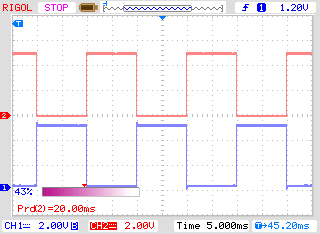
\includegraphics[]{../PNG/Frequency50.png}
\caption{Oscilogram \(50Hz\) výstupů portů 2 a 3}
\label{fig:Frequency50}
\end{figure}

Pokud pro generování taktu nepoužíváte krystal, můžou být výsledky měření kondenzátorů nepřesné.
Přesná frekvence taktu a přesné čekací doby jsou důležité pro stanovení hodnot kapacit.
Výstup  \(50Hz\) signálu lze předčasně zrušit přidržením tlačítka start.
Poté program pokračuje v normálním měření.

\subsection{Některé výsledky autotestu}

Výsledky autotestu 9 různých procesorů ATmega168 a 6 procesorů ATmega328
jsou uvedeny na následujících obrázcích. 

\begin{table}[H]
  \begin{center}
    \begin{tabular}{| l | c | c | c |}
    \hline
Test č. &  Typ měření    & Ideální hodnota & Obrázek \\
    \hline
    \hline
Test 1 & band gap Ref  & 1100 & \ref{fig:SelfTref} \\
    \hline
Test 2 & RL střed & 0 & \ref{fig:SelfTMitL} \\
    \hline
Test 3 & RH střed & 0 & \ref{fig:SelfTMitH} \\
    \hline
Test 5 & RH Low &  0 & \ref{fig:SelfTlowH} \\
    \hline
Test 6 & RH High & 0 & \ref{fig:SelfTtopH} \\
    \hline
Test 8 & R out Lo & 131 & \ref{fig:SelfTRoL} \\
    \hline
Test 9 & R out Hi & 151 & \ref{fig:SelfTRoH} \\
    \hline
Test 10 & Cap0  & 30 & \ref{fig:SelfTcap} \\
    \hline
Test 11 & korekce reference  & 0 & \ref{fig:SelfTrefKorr} \\
    \hline
    \end{tabular}
  \end{center}
  \caption{Seznam diagramů autotestu}
  \label{tab:test_m168} 
\end{table}

\begin{figure}[H]
  \centering
  \includegraphics[]{../GNU/SelfTrefCZ.pdf}
  \caption{Autotest: referenční napětí}
  \label{fig:SelfTref}
\end{figure}

\begin{figure}[H]
  \begin{subfigure}[b]{.5\textwidth}
    \centering
    \includegraphics[width=1.\textwidth]{../GNU/SelfTMitLCZ.pdf}
    \caption{s \(680 \Omega\)}
    \label{fig:SelfTMitL}
  \end{subfigure}
  ~
  \begin{subfigure}[b]{.5\textwidth}
    \centering
    \includegraphics[width=1.\textwidth]{../GNU/SelfTMitHCZ.pdf}
    \caption{s \(470 k\Omega\)}
    \label{fig:SelfTMitH}
  \end{subfigure}
  \caption{Autotest: odchylka středového napětí}
\end{figure}

\begin{figure}[H]
  \begin{subfigure}[b]{.5\textwidth}
  \centering
    \includegraphics[width=1.\textwidth]{../GNU/SelfTbottomHCZ.pdf}
    \caption{s \(470k\Omega\) na \(0V\)}
    \label{fig:SelfTlowH}
  \end{subfigure}
  ~
  \begin{subfigure}[b]{.5\textwidth}
  \centering
    \includegraphics[width=1.\textwidth]{../GNU/SelfTtopHCZ.pdf}
    \caption{s \(470k\Omega\) na \(5V\)}
    \label{fig:SelfTtopH}
  \end{subfigure}
  \caption{Autotest: vstupní napětí}
\end{figure}

\begin{figure}[H]
  \begin{subfigure}[b]{.5\textwidth}
  \centering
    \includegraphics[width=1.\textwidth]{../GNU/SelfTRiLoCZ.pdf}
    \caption{s \(680\Omega\) na \(5V\)}
    \label{fig:SelfTRoL}
  \end{subfigure}
  ~
  \begin{subfigure}[b]{.5\textwidth}
  \centering
    \includegraphics[width=1.\textwidth]{../GNU/SelfTRiHiCZ.pdf}
    \caption{s \(680\Omega\) na \(0V\)}
    \label{fig:SelfTRoH}
  \end{subfigure}
  \caption{Autotest: výstupní odpor}
\end{figure}

\begin{figure}[H]
  \centering
  \includegraphics[width=.6\textwidth]{../GNU/SelfTcap0CZ.pdf}
  \caption{Autotest: nulová hodnota měření kapacity}
  \label{fig:SelfTcap}
\end{figure}

\begin{figure}[H]
  \centering
  \includegraphics[width=.6\textwidth]{../GNU/SelfTrefKorrCZ.pdf}
  \caption{Autotest: hodnoty automatické korekce kalibrace}
  \label{fig:SelfTrefKorr}
\end{figure}

Ke konci bych chtěl ukázat rozdíly na pinu AREF měřených napětí pomocí multimetru
a vnitřně měřených s referenčních ADC napětí 15 různých ATmegas a těch s automaticky
nastavených (REF\_R\_KORR)  korektur, který se nachází na obrázku\ref{fig:SelfTrefDiff}.
Zde je vidět, že hodnoty automatické kalibrace jsou téměř stejné jako hodnoty externích měřidel a
následovně naměřených referenčních hodnot napětí.
\begin{figure}[H]
  \centering
  \includegraphics[width=.6\textwidth]{../GNU/SelfTrefDiffCZ.pdf}
  \caption{Autotest: rozdíl napětí v interní referenci}
  \label{fig:SelfTrefDiff}
\end{figure}

